\documentclass[tikz,border=10pt]{standalone}
\usepackage{amsmath}
\usepackage{tikz}
\usetikzlibrary{arrows.meta, positioning, calc, shapes.geometric}

\begin{document}
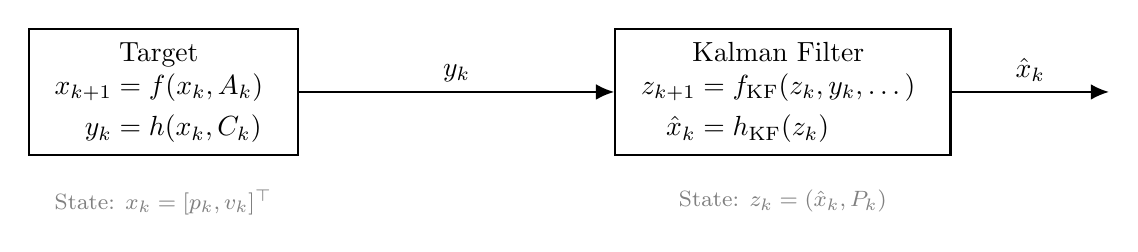
\begin{tikzpicture}[
  block/.style = {draw, thick, minimum height=3em, minimum width=6em, align=center},
  arrow/.style = {thick, -{Latex[width=2mm]}},
  node distance=2.5cm and 4cm
]

  % Target block (system being tracked)
  \node[block] (target) {
    \begin{tabular}{c}
      Target\\
      $\begin{aligned}
        x_{k+1} &= f(x_k, A_k) \\
        y_k &= h(x_k, C_k)
      \end{aligned}$
    \end{tabular}
  };

  % Kalman Filter block
  \node[block, right=of target] (kf) {
    \begin{tabular}{c}
      Kalman Filter\\
      $\begin{aligned}
        z_{k+1} &= f_{\text{KF}}(z_k, y_k, \dots) \\
        \hat{x}_k &= h_{\text{KF}}(z_k)
      \end{aligned}$
    \end{tabular}
  };

  % Measurement flow: target -> KF
  \draw[arrow] (target.east) -- node[above] {$y_k$} (kf.west);

  % State estimate output from KF
  \draw[arrow] (kf.east) -- ++(2,0) node[midway, above] {$\hat{x}_k$};

  % Labels below blocks
  \node[below=0.3cm of target, font=\footnotesize, text=gray] {State: $x_k = [p_k, v_k]^\top$};
  \node[below=0.3cm of kf, font=\footnotesize, text=gray] {State: $z_k = (\hat{x}_k, P_k)$};

\end{tikzpicture}
\end{document}
